\documentclass[11pt]{article}
\usepackage[T1]{fontenc}
\usepackage[utf8]{inputenc}
\usepackage[french]{babel}
\usepackage[margin=2.5cm]{geometry}
\usepackage{graphicx}
\usepackage{mathptmx}
\usepackage{setspace}
\usepackage{titlesec} 
\usepackage{imakeidx} 
\usepackage{tcolorbox}
\usepackage{caption}

\setlength{\parindent}{1cm}
\makeindex
\renewcommand{\rmdefault}{ptm}
\onehalfspacing % Interligne de 1.5
\setcounter{page}{1}
\titleformat{\section}
{\fontsize{16}{19}\selectfont\bfseries} 
{\thesection}
{20pt}
{}

\titleformat{\subsection}
{\fontsize{15}{19}\selectfont\bfseries} 
{\thesubsection}
{20pt}
{}

\renewcommand{\theparagraph}{\thesubsubsection.\arabic{paragraph}}
\titleformat{\paragraph}
{\normalfont\normalsize\bfseries}{\theparagraph}{1em}{}

% \makeatletter
% \renewcommand{\paragraph}{%
%   \@startsection{paragraph}{4}%
%   {\z@}{3.25ex \@plus1ex \@minus.2ex}{-1em}%
%   {\normalfont\normalsize\bfseries}%
% }
% \makeatother

\begin{document}
\pagenumbering{gobble} % Supprime la numérotation des pages
\begin{titlepage}
    \begin{center}

        \begin{minipage}[b]{0.3\textwidth}
            
\includegraphics[width=\textwidth]{images/Logo_Universite_de_Lorraine.png}
        \end{minipage}
        \begin{minipage}[b]{0.2\textwidth}
            \centering
            
\includegraphics[width=\textwidth]{images/logo-fst-format-jpg-couleur.jpg}
        \end{minipage}
        \smallbreak
        \vspace{0.5cm}
        \textbf{\large Master Informatique}

        %% Milieu de la page
        \vfill
        {\Large Reconnaissance des mouvements de la main} \smallbreak
        Rapport \smallbreak en vue de la validation de l'UE Initiation à la recherche \smallbreak
        \vfill
        \begin{tabular}{ccc|ccc}
            \'Etudiants : & Victor DALL\'E &  &  & Encadrante : & Madame BOLTCHEVA \\
                          & Claire KURTH   &  &  &              &
        \end{tabular}
    \end{center}

\end{titlepage}

\newpage \newpage
\section*{Décharge de responsabilité }\bigbreak
L'Université de Lorraine n'entend donner ni approbation  ni improbabtion aux opinions émises dans ce rapport,
ces opinions devant être considérées comme propres à leurs auteurs. \bigbreak

\newpage
\section*{Remerciements}

\newpage
\tableofcontents
\newpage

\pagenumbering{arabic}
\setcounter{page}{1}
\section*{Introduction}
\addcontentsline{toc}{section}{Introduction}
De nos jours, la vision par ordinateur est un domaine en plein essor. La reconnaissance de gestes fait partie intégrante de ce domaine et à ce titre, incarne une révolution dans la manière dont les utilisateurs interagissent avec les systèmes informatiques. Cette technologie est en effet en train de transformer la façon dont nous interagissont avec les machines. Cette avancée offre des opportunités novatrices dans des domaines tels que l'interaction entre l'homme et la machine,
la réalité augmentée ou encore l'accessibilité numérique.
De nombreuses techniques existent déjà pour permettre la détection des mains. MediaPipe de Google [src] utilise le machine learning pour entrainer un modèle qui détecte les segments composant la main. D'autres travaux ont été réalisés comme ceux de l'équipe du professeur Kalpana Joshi [src] qui utilise les angles formés entre 2 doigts pour détecter la forme de la main (nombre de doigts, main ouverte ou fermée).\bigbreak

Contrairement aux interfaces traditionnelles basées sur le clavier et la souris, la reconnaissance des gestes permet aux utilisateurs de communiquer plus simplement avec les ordinateurs. Ils peuvent désormais avoir recours à leurs mains ou à leur corps pour contrôler les applications, ou encore naviguer dans des environnements virtuels. Cette approche favorise une expérience utilisateur plus immersive et ergonomique, ouvrant ainsi de nouvelles perspectives dans des domaines variés tels que le divertissement interactif, l'éducation, ou encore la médecine. Comme dit précédemment, la reconnaissance des mouvements joue un rôle crucial dans l’accessibilité numérique en permettant à des personnes porteuses d'un handicap physique  ou moteur de pouvoir communiquer et d'interagir avec des outils numériques plus facilement. En effet, celà permet de passer outre les obstacles liés à l’utilisation des outils traditionnels (tels que le clavier, la souris, la télécommande …) grâce à la simple utilisation de mouvements du corps. Cette nouvelle manière d'interagir avec un système numérique est déjà utilisée dans plusieurs domaines notamment le sport avec des applications de coaching personnel qui permettent de suivre les mouvements de l'utilisateur et ainsi lui donner des conseils pour améliorer sa technique, ou encore sa posture. Ce nouveau concept d'interraction permet également de pouvoir contrôler des appareils tels que des téléviseurs où par un simple geste, nous pouvons par exemple gérer le son ou changer de chaîne. \bigbreak

Dans ce contexte, ce projet vise à se questionner vis-à-vis d'un système de reconnaissance des mouvements de la main à l’aide d’un classifieur classique Haar-cascade et de le comparer avec un système de reconnaissance de la main sans classifieur.
L'objectif principal est de concevoir un système capable de détecter et de classifier différents gestes de la main effectués par l'utilisateur,
tels que le poing fermé, ou alors la main ouverte avec un certains nombre de doigts levés. Ces gestes seront ensuite associés à différentes
actions telles que le lancement d'applications ou encore l'ouverture de sites web.
Pour réaliser ce projet nous utiliserons principalement la bibliothèque OpenCV. Nous parlerons dans un premier temps plus en détail des techniques de reconnaissance de gestes actuellement utilisées, puis nous expliciterons les notions techniques ainsi que les méthodes que nous exploiterons. Nous verrons ensuite comment nous avons implémenté la reconnaissance de la main sans le classifieur classique Haar-Cascade puis avec ce classifieur.

\newpage

\section{Rappel du sujet et encadrement}
\subsection{Rappel du sujet}

Le but de ce projet est d’implémenter un système de reconnaissance des mouvements de la
main à l’aide d’un classifieur classique Haar-cascade. Le système doit reconnaître le geste de
la main de l’utilisateur (poing, un doigt, deux, trois, quatre,...) et le mapper à différentes tâches
telles que le lancement d’applications comme le bloc-notes, la peinture, et l’ouverture de sites web.
Le système doit être mis en œuvre avec l’aide de la librairie de "Computer Vision" - OpenCV,
comme dans l’article [src]. Une extension possible serait l’implémentation d’un système de détection
des mouvements de la tête ou du corps, tout entier.

\subsection{Encadrement}

\newpage

\section{\'Etat de l'art}
\subsection{Article de départ}
\subsection{Médiapipe}
Médiapipe est un framework open-source développé par Google permettant de construire des pipelines de traitement de données multimédia. Il propose des solutions pour la détection de la main, du visage ou encore de la pose. Il est basé sur des modèles de machine learning notamment grâce à de l'apprentissage via des réseaux de neurones. \bigbreak

[Image de la main détectée par Médiapipe]


\subsection{classifieur classique Haar-cascade}
Le classifieur Haar-cascade est une méthode de détection d'objets dans une image introduit par Paul Viola et Michael Jones en 2001 [src]. Il est basé sur l'utilisation de caractéristiques de type Haar. Ces caractéristiques sont des fenêtres de taille fixe qui sont déplacées sur l'image et qui permettent de calculer la différence de luminosité entre les pixels de la fenêtre. Ces caractéristiques sont ensuite utilisées pour entraîner un classifieur qui permet de détecter des objets dans une image. \bigbreak

Les classifieurs Haar-cascade sont utilisés pour la détection de visages, de voitures, de plaques d'immatriculation, de piétons, de mains ou de tout autres objets. Ils sont très utilisés dans le domaine de la vision par ordinateur et sont très efficaces pour la détection d'objets dans une image. \bigbreak



\newpage

\section{Reconnaissance de la main avec classifieur classique Haar-cascade}
\subsection{Entrainer un classifieur Haar-cascade}
Pour entrainer un classifieur Haar-cascade, il faut tout d'abord collecter des images positives et négatives. Les images positives sont des images contenant l'objet que l'on souhaite détecter, tandis que les images négatives sont des images ne contenant pas l'objet. Il faut ensuite générer des fichiers de descriptions des images positives et négatives. Ces fichiers contiennent les coordonnées des objets à détecter dans les images positives. Enfin, il faut entrainer le classifieur à l'aide de ces fichiers de descriptions. \bigbreak

L'entrainement du classifieurs en lui-même se fait grâce à ce que l'on appelle des "features". Ces dernières ont été introduites par Viola et Jones en 2001 (Fig. \ref{fig:haar_features_1}). Par la suite, d'autres features ont été ajoutées (Fig. \ref{fig:haar_features_2}) afin d'améliorer la détection d'objets dans une image.
\bigbreak \bigbreak

\begin{minipage}[t]{0.35\textwidth}
    \begin{center}
        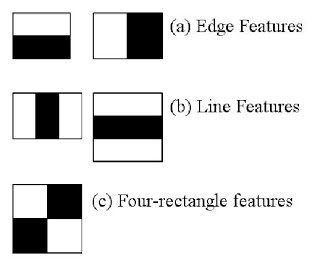
\includegraphics[width=\textwidth]{images/haar_features.jpg}  
        \captionof{figure}{Features de Haar comme utilisées par Viola et Jones.} 
        \label{fig:haar_features_1}
    \end{center} 
\end{minipage}\hspace{1.5cm}
\begin{minipage}[t]{0.45\textwidth}
    \begin{center}
        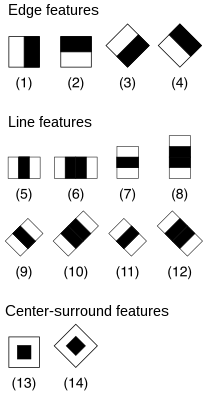
\includegraphics[width=0.8\textwidth]{images/haar_feature_2.jpg}
        \captionof{figure}{Features de Haar supplémentaires.}
        \label{fig:haar_features_2}
    \end{center}
\end{minipage}

\bigbreak \bigbreak


Ces features sont des caractéristiques de l'objet que l'on souhaite détecter, ce sont des patterns de pixels qui permettent de distinguer l'objet des autres éléments de l'image.

\noindent Il existe différents types de patterns :
\begin{itemize}
    \item Les "edges" : ce sont des patterns qui permettent de détecter les contours de l'objet.
    \item Les "lines" : ce sont des patterns qui permettent de détecter les lignes de l'objet.
    \item Les "center-surrounder" : ce sont des patterns qui permettent de détecter les changements d'intensité entre le centre d'une région rectangulaire et le reste de la région. Cela permet de détecter des objets de forme particulière.
\end{itemize}



\bigbreak

Ces features sont ensuite utilisées pour entrainer un classifieur qui permet de détecter l'objet dans une image. Le classifieur est entrainé à l'aide d'un algorithme de machine learning tel que AdaBoost qui permet de déterminer les features les plus pertinentes pour la détection de l'objet. \bigbreak

AdaBoost est un algorithme d'apprentissage supervisé qui permet de construire un classifieur fort à partir de plusieurs classifieurs faibles. 
Au début, chaque élément de la base de données à le même poids. L'algorithme va ensuite sélectionner un classifieur faible (par exemple, un arbre de décision simple) qui performe légèrement mieux que l'aléatoire. Ce classifieur va être utilisé pour prédire les éléments de la base de données. Les exemples mal classés reçoivent un poids plus élevé, tandis que les exemples correctement classés reçoivent un poids plus faible. Ainsi, les exemples difficiles à classer ont plus d'influence sur la formation du classifieur final. Les poids des classifieurs faibles sont déterminés en fonction de leur précision relative. Les classifieurs les plus précis ont un poids plus élevé. Enfin, le classifieur final est une combinaison linéaire des classifieurs faibles pondérés par leur précision relative. \bigbreak


[Src : https://www.almabetter.com/bytes/tutorials/data-science/adaboost-algorithm]

\subsection{Nos entrainements}
\subsubsection{Avec une base de données d'images de mains}
\paragraph{Méthodologie}
Pour notre entrainement, nous avons collecté 10 000 images négatives et 5 000 images positives de mains. Pour les images positives, nous avons ensuite utilisé la librairie OpenCV pour générer les fichiers de descriptions des images positives. Les fichiers de descriptions contiennent les coordonnées des mains dans les images positives. Nous avons ensuite entrainé le classifieur à l'aide de ces fichiers de descriptions. \'Etant donné que les images positives ne contenaient que la main, la description comprenait la taille et la hauteur de l'image. \bigbreak

Nous sommes ensuite passés à l'entrainement. Nous avons utilisé pour celà OpenCV qui propose un programme pour entrainer un classifieur Haar-cascade. Nous avons testé plusieurs cas : avec 5, 10, 15 et 20 étapes, avec des profondeurs d'arbres maximum différentes, avec plus d'images positives que négatives et vice-versa. Enfin, avons aussi testé le nombre de "Faux positif" maximum autorisé, c'est-à-dire le nombre maximum d'images négatives mal classées autorisées. \bigbreak 

Faire un tab récap pour les heures ??? \bigbreak

\paragraph{Résultats}

\paragraph{Conclusion}
Les résultats ne sont pas entièrement satisfaisant. En effet, le classifieur ne détecte pas toute la main mais seulement plusieurs parties de la main. Celà est certainement dû au fait que les images positives ne contienent que la main sans "background" et que les features utilisées ne sont pas suffisamment pertinentes pour détecter la main dans une image. \bigbreak

\subsubsection{En créant nous même des images positives}
\paragraph{Méthodologie}
N'ayant pas obtenus de résultats satisfaisants avec la base de données d'images de mains, nous avons décidé de créer nous même des images positives. Pour cela, nous avons utilisé la librairie OpenCV pour ajouter une image de main aux images positives. Nous avons ensuite généré les fichiers de descriptions des images positives et entrainé le classifieur à l'aide de ces fichiers. \bigbreak


[Photo ex neg et pos]

\paragraph{Résultats}

\paragraph{Conclusion}
Les résultats ne sont pas beaucoup plus satisfaisant. On obtient les mêmes résultats que précédemment. \bigbreak

Il faudrait essayer de prendre une base de données de mains contenant des background différents et annoter les images pour voir si celà améliore les résultats. \bigbreak


\section{Reconnaissance de la main sans classifieur}
\subsection{Méthodologie}
Pour réussir à détecter la main sans classifieur, nous avons dû tester plusieurs méthodes. En effet, plusieurs paramètres interviennent afin d'avoir une détection de la main optimale. 

On a dû jouer sur plusieurs paramètres : 
\begin{itemize}
    \item Le format de la couleur de l'image : GreyScale ou HSV
    \item Flou : avec ou sans, quel type de flou (Gaussien ou Bilatéral)
    \item Thresholding : pour binariser l'image. Il y avait là plusieurs paramètres possibles : le seuil et le type de thresholding (binaire, binaire inversé, tronqué, to zero, to zero inversé)
\end{itemize}

\subsection{Expériences et résultats}
Pour trouver les meilleures paramètres, nous avons testé plusieurs combinaisons de paramètres. 

blablabla

\subsection{Détection des doigts}


\newpage

\section{Fusion des deux systèmes}
\subsection{Méthodologie}
Nous avons un classifieur d'une part qui détecte une portion de la main et d'autres part un système qui permet de détecter la main si on a bien configuré les paramètres. Nous allons donc fusionner ces deux systèmes : si le classifieur détecte une portion de la main, on utilise la plus grande portion de la main détectée afin de récupéré tout d'abord la couleur de la main puis 
\subsection{Expériences et résultats}
\subsection{Conclusion}
\newpage

\section*{Conclusion}
\addcontentsline{toc}{section}{Conclusion}
\newpage

\section*{Annexes}
\addcontentsline{toc}{section}{Annexes}

\section*{Bibliographie}
\addcontentsline{toc}{section}{Bibliographie}
\newpage

\section*{Glossaire}

\section*{Déclaration sur l'honneur contre le plagiat}

\newpage

\newpage
\section*{Résumé}

\end{document}